\documentclass[../main/main.tex]{subfiles}

\newdate{date}{16}{10}{2019}

\begin{document}


\marginpar{ \textbf{Lecture 3.} \\  \displaydate{date}. \\ Compiled:  \today.}


\section{Lever Rule}
Consider the Figure \ref{fig:3_0}, at all points between \emph{A} and \emph{B} the system is a mixsture of gas and liquid. Points \emph{D} has global density \( P_D = P_A + P_B \)  and therefore \( v_D = \frac{1}{P_D}, v_A = \frac{1}{P_A}, v_B = \frac{1}{P_B} \) which implies:
\begin{equation}
  v_D = \frac{N_A}{N} v_A + \frac{N_B}{N} v_B = x_A v_A + x_B v_B
  \label{eq:}
\end{equation}
Since \( x_A + x_B = 1 \) we have \( (x_A + x_B)v_D = x_A v_A + x_B v_B \) and finally the \textbf{Lever Rule}:
\begin{equation}
  \frac{x_A}{x_B} = \frac{v_B - v_D}{v_D - v_A}
  \label{eq:}
\end{equation}
\begin{figure}[h!]
\centering



\tikzset{every picture/.style={line width=0.75pt}} %set default line width to 0.75pt

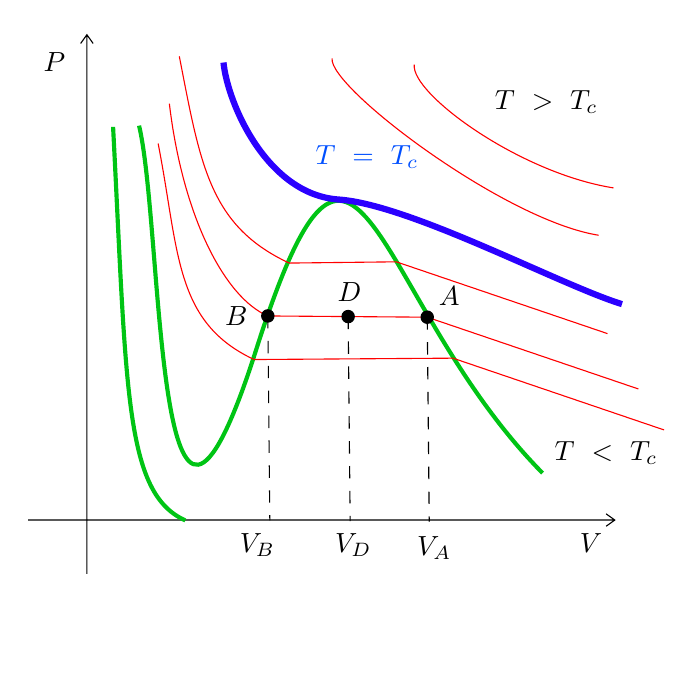
\begin{tikzpicture}[x=0.75pt,y=0.75pt,yscale=-0.6,xscale=0.6]
%uncomment if require: \path (0,433); %set diagram left start at 0, and has height of 433

%Shape: Axis 2D [id:dp34042133393206886]
\draw  (72,390.7) -- (543,390.7)(119.1,1) -- (119.1,434) (536,385.7) -- (543,390.7) -- (536,395.7) (114.1,8) -- (119.1,1) -- (124.1,8)  ;
%Straight Lines [id:da6702336744569144]
\draw  [dash pattern={on 4.5pt off 4.5pt}]  (264.39,226.81) -- (266,391) ;


%Straight Lines [id:da35901728946704126]
\draw [color={rgb, 255:red, 255; green, 0; blue, 0 }  ,draw opacity=1 ]   (263.39,226.81) -- (392.39,227.81) ;


%Curve Lines [id:da9451173727045867]
\draw [color={rgb, 255:red, 0; green, 196; blue, 21 }  ,draw opacity=1 ][line width=1.5]    (161,74) .. controls (181,159) and (173,511) .. (255,254) .. controls (337,-3) and (347,213) .. (485,353) ;


%Straight Lines [id:da08613827611481972]
\draw  [dash pattern={on 4.5pt off 4.5pt}]  (392.39,227.81) -- (394,392) ;


%Straight Lines [id:da1041450850592075]
\draw [color={rgb, 255:red, 255; green, 0; blue, 0 }  ,draw opacity=1 ]   (281.55,184.35) -- (367.55,183.35) ;


%Straight Lines [id:da726756834820412]
\draw [color={rgb, 255:red, 255; green, 0; blue, 0 }  ,draw opacity=1 ]   (253.39,261.81) -- (413.01,260.71) ;


%Straight Lines [id:da36415288687545777]
\draw  [dash pattern={on 4.5pt off 4.5pt}]  (328.89,227.31) -- (330.5,391.5) ;


%Curve Lines [id:da6577640934100049]
\draw [color={rgb, 255:red, 255; green, 0; blue, 0 }  ,draw opacity=1 ]   (193.31,18.33) .. controls (210.31,105.33) and (217.31,154.33) .. (281.55,184.35) ;


%Curve Lines [id:da5326240116615772]
\draw [color={rgb, 255:red, 255; green, 0; blue, 0 }  ,draw opacity=1 ]   (176.31,88.33) .. controls (193.31,175.33) and (189.15,231.78) .. (253.39,261.81) ;


%Curve Lines [id:da7998397977403133]
\draw [color={rgb, 255:red, 255; green, 0; blue, 0 }  ,draw opacity=1 ]   (185.31,56.33) .. controls (196.31,148.33) and (230.31,212.33) .. (264.39,226.81) ;


%Straight Lines [id:da9411455399902455]
\draw [color={rgb, 255:red, 255; green, 0; blue, 0 }  ,draw opacity=1 ]   (367.55,183.35) -- (537.13,240.99) ;


%Straight Lines [id:da28743856092342424]
\draw [color={rgb, 255:red, 255; green, 0; blue, 0 }  ,draw opacity=1 ]   (392.39,227.81) -- (561.97,285.45) ;


%Straight Lines [id:da2729807224373272]
\draw [color={rgb, 255:red, 255; green, 0; blue, 0 }  ,draw opacity=1 ]   (413.01,260.71) -- (582.59,318.35) ;


%Curve Lines [id:da846663436815342]
\draw [color={rgb, 255:red, 0; green, 196; blue, 21 }  ,draw opacity=1 ][line width=1.5]    (140.13,74.99) .. controls (151.13,285.99) and (149.13,368.99) .. (198.13,390.99) ;


%Curve Lines [id:da687077505482324]
\draw [color={rgb, 255:red, 43; green, 0; blue, 255 }  ,draw opacity=1 ][line width=2.25]    (228.79,23.31) .. controls (232.09,56.31) and (263.8,129.35) .. (321.29,133.33) .. controls (378.79,137.31) and (499.79,202.31) .. (548.79,217.31) ;


%Shape: Circle [id:dp9253191380995789]
\draw  [color={rgb, 255:red, 0; green, 0; blue, 0 }  ,draw opacity=1 ][fill={rgb, 255:red, 0; green, 0; blue, 0 }  ,fill opacity=1 ] (323.94,227.31) .. controls (323.94,224.57) and (326.15,222.35) .. (328.89,222.35) .. controls (331.63,222.35) and (333.84,224.57) .. (333.84,227.31) .. controls (333.84,230.04) and (331.63,232.26) .. (328.89,232.26) .. controls (326.15,232.26) and (323.94,230.04) .. (323.94,227.31) -- cycle ;
%Shape: Circle [id:dp4312182648745586]
\draw  [color={rgb, 255:red, 0; green, 0; blue, 0 }  ,draw opacity=1 ][fill={rgb, 255:red, 0; green, 0; blue, 0 }  ,fill opacity=1 ] (259.44,226.81) .. controls (259.44,224.07) and (261.65,221.85) .. (264.39,221.85) .. controls (267.13,221.85) and (269.34,224.07) .. (269.34,226.81) .. controls (269.34,229.54) and (267.13,231.76) .. (264.39,231.76) .. controls (261.65,231.76) and (259.44,229.54) .. (259.44,226.81) -- cycle ;
%Shape: Circle [id:dp9164322895828938]
\draw  [color={rgb, 255:red, 0; green, 0; blue, 0 }  ,draw opacity=1 ][fill={rgb, 255:red, 0; green, 0; blue, 0 }  ,fill opacity=1 ] (387.44,227.81) .. controls (387.44,225.07) and (389.65,222.85) .. (392.39,222.85) .. controls (395.13,222.85) and (397.34,225.07) .. (397.34,227.81) .. controls (397.34,230.54) and (395.13,232.76) .. (392.39,232.76) .. controls (389.65,232.76) and (387.44,230.54) .. (387.44,227.81) -- cycle ;
%Curve Lines [id:da7173087694815479]
\draw [color={rgb, 255:red, 255; green, 0; blue, 0 }  ,draw opacity=1 ]   (316,20) .. controls (313,43) and (454,150) .. (530,162) ;


%Curve Lines [id:da07422455776903614]
\draw [color={rgb, 255:red, 255; green, 0; blue, 0 }  ,draw opacity=1 ]   (382,25) .. controls (379,48) and (466,112) .. (542,124) ;



% Text Node
\draw (93,23) node   {$P$};
% Text Node
\draw (524,409) node   {$V$};
% Text Node
\draw (256,411) node   {$V_{B}$};
% Text Node
\draw (398,413) node   {$V_{A}$};
% Text Node
\draw (333,411) node   {$V_{D}$};
% Text Node
\draw (239,227) node   {$B$};
% Text Node
\draw (410,211) node   {$A$};
% Text Node
\draw (330,208) node   {$D$};
% Text Node
\draw (344,99) node [color={rgb, 255:red, 0; green, 79; blue, 255 }  ,opacity=1 ]  {$T\ =\ T_{c}$};
% Text Node
\draw (488,55) node   {$T\  >\ T_{c}$};
% Text Node
\draw (536,337) node   {$T\ < \ T_{c}$};


\end{tikzpicture}

\caption{\label{fig:3_0} Description.}
\end{figure}

\section{Thermodynamic of phase coexistence (one component system)}
Consider a \( (P,V,T) \) system as a mixture of two species \( (1,2) \) at temperature \( T_1, T_2 \), pressure \( P_1, P_2 \) and chemical potentials \( \mu _1,\mu _2 \). The equilibrium condition is given by the maximum of the total entropy \( S = S_1 + S_2 \) and gives the conditions
\begin{equation}
  T_1 = T_2, \quad P_1 = P_2, \quad \mu _1 = \mu _2
  \label{eq:}
\end{equation}
this is the \emph{coexistence condition} of the two phases.
In terms of the Gibbs potential \( G = U- TS+PV \), where \emph{U} is given by  the Euler equation \( U = TS-PV+ \mu _1 N_1 + \mu _2 N_2 \), the Gibbs per mole is
\begin{subequations}
\begin{align}
  g_1 (T,P) &\equiv \frac{G_1}{N_1} = \mu _1 \\
  g_2 (T,P) &\equiv \frac{G_2}{N_2} = \mu _2
\end{align}
\label{}
\end{subequations}
Therefore, on the coexistence line it should hold the relation
\begin{equation}
  g_1 (T,P) = g_2 (T,P)
  \label{eq:}
\end{equation}

\section{Clausius-Clapeyron equation}
Suppose to know the position an the coexistence line (for example the melt temperature \( T_m \) at the atmospheric pressure \( P_0 \), as in Figure \ref{fig:3_1}  ). Is it possible to find other points on the curve? For example \( T_m \) at lower or higher pressure ?


\begin{figure}[h!]
\centering


\tikzset{every picture/.style={line width=0.75pt}} %set default line width to 0.75pt

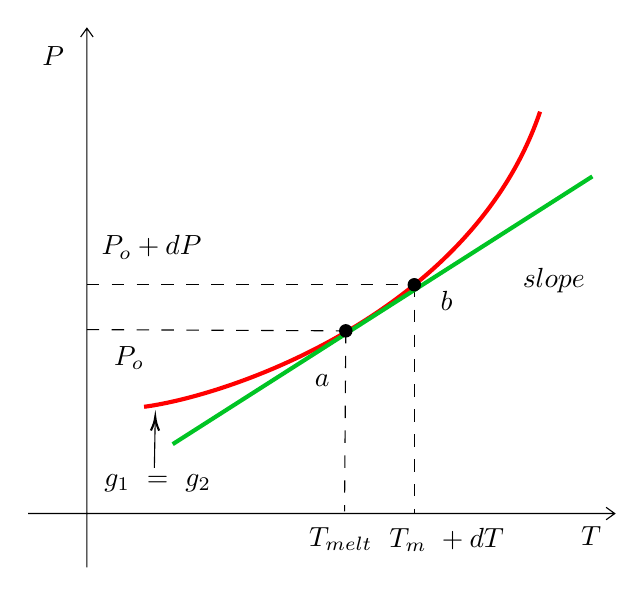
\begin{tikzpicture}[x=0.75pt,y=0.75pt,yscale=-0.6,xscale=0.6]
%uncomment if require: \path (0,433); %set diagram left start at 0, and has height of 433

%Shape: Axis 2D [id:dp34042133393206886]
\draw  (72,390.7) -- (543,390.7)(119.1,1) -- (119.1,434) (536,385.7) -- (543,390.7) -- (536,395.7) (114.1,8) -- (119.1,1) -- (124.1,8)  ;
%Straight Lines [id:da6702336744569144]
\draw  [dash pattern={on 4.5pt off 4.5pt}]  (327,244) -- (326,389) ;


%Straight Lines [id:da7053989083670136]
\draw  [dash pattern={on 4.5pt off 4.5pt}]  (382,207) -- (382,390) ;


%Curve Lines [id:da6886563534922254]
\draw [color={rgb, 255:red, 255; green, 0; blue, 0 }  ,draw opacity=1 ][line width=1.5]    (165,305) .. controls (239,295) and (429,227) .. (483,68) ;


%Straight Lines [id:da01620685432223168]
\draw  [dash pattern={on 4.5pt off 4.5pt}]  (119,243) -- (327,244) ;


%Straight Lines [id:da6787352217788557]
\draw  [dash pattern={on 4.5pt off 4.5pt}]  (119,207) -- (382,207) ;


%Straight Lines [id:da3303084254473059]
\draw [color={rgb, 255:red, 0; green, 196; blue, 36 }  ,draw opacity=1 ][line width=1.5]    (188,335) -- (525,120) ;


%Shape: Circle [id:dp23372095277787042]
\draw  [color={rgb, 255:red, 0; green, 0; blue, 0 }  ,draw opacity=1 ][fill={rgb, 255:red, 0; green, 0; blue, 0 }  ,fill opacity=1 ] (377.05,207) .. controls (377.05,204.26) and (379.26,202.05) .. (382,202.05) .. controls (384.74,202.05) and (386.95,204.26) .. (386.95,207) .. controls (386.95,209.74) and (384.74,211.95) .. (382,211.95) .. controls (379.26,211.95) and (377.05,209.74) .. (377.05,207) -- cycle ;
%Shape: Circle [id:dp06058395143705542]
\draw  [color={rgb, 255:red, 0; green, 0; blue, 0 }  ,draw opacity=1 ][fill={rgb, 255:red, 0; green, 0; blue, 0 }  ,fill opacity=1 ] (322.05,244) .. controls (322.05,241.26) and (324.26,239.05) .. (327,239.05) .. controls (329.74,239.05) and (331.95,241.26) .. (331.95,244) .. controls (331.95,246.74) and (329.74,248.95) .. (327,248.95) .. controls (324.26,248.95) and (322.05,246.74) .. (322.05,244) -- cycle ;
%Straight Lines [id:da4596906688697088]
\draw    (173.28,353.97) -- (173.96,315.12) ;
\draw [shift={(174,313.12)}, rotate = 451] [color={rgb, 255:red, 0; green, 0; blue, 0 }  ][line width=0.75]    (10.93,-3.29) .. controls (6.95,-1.4) and (3.31,-0.3) .. (0,0) .. controls (3.31,0.3) and (6.95,1.4) .. (10.93,3.29)   ;


% Text Node
\draw (92,23) node   {$P$};
% Text Node
\draw (524,409) node   {$T$};
% Text Node
\draw (323,411) node   {$T_{melt}$};
% Text Node
\draw (408,412) node   {$T_{m} \ +dT$};
% Text Node
\draw (153,266) node   {$P_{o}$};
% Text Node
\draw (171,177) node   {$P_{o} +dP$};
% Text Node
\draw (308,284) node   {$a$};
% Text Node
\draw (408,220) node   {$b$};
% Text Node
\draw (494,204) node   {$slope$};
% Text Node
\draw (176,366.2) node   {$g_{1} \ =\ g_{2}$};


\end{tikzpicture}

\caption{\label{fig:3_1} Description.}
\end{figure}

The answer is yes for small deviations of \emph{T} and \emph{P} from \emph{a}. Rhe idea is to compute the slope of the tangent of the coexistence curve, i.e. \( (\dd[]{P}/\dd[]{T}  )  \). This is given by the Clausius-Clapeyron equation.
Both at \emph{a} and \emph{b} the two phases 1 and 2 coexist. This means  that at the coexistence line
\begin{equation}
  \begin{cases}
   g_1^{(a)} = g_2^{(a)}\\
   g_1^{(b)} = g_2^{(b)}
  \end{cases}
\label{eq:}
\end{equation}
Hence, if \emph{a} and \emph{b} are very close:
\begin{equation}
  \begin{cases}
  \dd[]{g_1} = g_1^{(b)} - g_1^{(a)} \\
  \dd[]{g_2} = g_2^{(b)} - g_2^{(a)}
  \end{cases}
\label{eq:}
\end{equation}
Therefore, the \emph{starting point} for \emph{Clausius-Clapeyron} is
\begin{equation}
  \Rightarrow \dd[]{g_1} =\dd[]{g_2}
  \label{eq:}
\end{equation}
From the molar version of the Gibbs-Duhem relation we have
\begin{equation}
  \begin{cases}
   \dd[]{g_1} = -s_1 \dd[]{T} + v_1 \dd[]{P} = \dd[]{\mu _1}    \\
   \dd[]{g_2} = -s_2 \dd[]{T} + v_2 \dd[]{P} = \dd[]{\mu _2}
  \end{cases}
\label{eq:}
\end{equation}
taking the difference, one obtains
\begin{equation}
  -(s_2 - s_1) \dd[]{T} + (v_2 - v_1) \dd[]{P} = 0
  \label{eq:}
\end{equation}
The splope is called \textcolor{blue}{\textbf{Clausius-Clapeyron equation}}:
\begin{empheq}[box=\myyellowbox]{equation}
  \qty(\dv{P}{T} )_{coex} = \frac{(s_2-s_1)}{(v_2-v_1)} = \frac{\Delta s}{\Delta v}
  \label{eq:}
\end{empheq}
\begin{remark}
Since \( (\dd[]{P}/\dd[]{T})_{coex}   \) is finite, the equation explains why a first order transition is characterised by discontinuous changes in entropy and volume (or density). \( \Delta S \)  gives the heat \( L_{12} \) that is exchanged with the environment:
\begin{equation}
  L_{12} = \Delta S T
  \label{eq:}
\end{equation}
\end{remark}

\subsection{Application of C-C equation to the liquid-gas coexistence line}
 Now, we go from gas to liquid (we call it respectively region 2 and 1), we have:

\begin{equation}
  \qty(\dv{P}{T} )_{coex} = \frac{s_2 - s_1}{v_2 - v_1}
  \label{eq:}
\end{equation}
Since for liquid-gas :
\begin{equation}
  \qty(\dv{P}{T} )_{coex} > 0 \Rightarrow \frac{s_2 - s_1}{v_2 - v_1} > 0
  \label{eq:}
\end{equation}
and since \( v_2 > v_1 \), we have \( s_2 > s_1 \). The gas has more entropy as it should be. When going from a low-temperature phase to a high-temperature phase entropy always increases \( \Delta S > 0 \), because \( c_P \equiv T (\partial{S}/\partial{T}  )_P > 0 \).

The sign of \( \Delta V \) is more uncertain though. To see this point let us consider the C-C equation at the solid-liquid (now solid is region 1 and liquid region 2) coexistence curve.
At the melt temperature:
\begin{equation}
  \qty(\dv{P}{T} )_{coex} = \frac{\delta Q_{melt}}{T_{melt}\Delta v_{melt}} \qquad \delta Q_{melt} = Q_{liq} - Q_{solid} > 0
  \label{eq:}
\end{equation}
In general, \( \Delta v_m = v_{liq} - v_{solid} > 0 \) which implies \( \qty( \dd[]{P}/\dd[]{T}   )_{coex} > 0  \). There are cases, however, where \( \Delta v_m = v_{liq} - v_{solid} < 0 \) because \( \rho_{liq} > \rho _{solid} \) (for instance the \( H_2 0 \), or also Silicon and Germanium). The paradigmatic example is the freezing of water where \( v_{ice} > v_{liq} \) since ice is less dense than liquid water at the coxistence (\( 0 < T° < 4 \) ). This implies that \( \dd[]{P}/\dd[]{T} < 0   \).

\begin{example}[Melting point on Everest] \

Consider \( T = 237 K \) and \( P=P_0 \). If \( \delta Q_m = 6.01 kJ/mol \) and \( \Delta v = -1.7 cm^3 /mol  \) we have:
\begin{equation}
  \dv{P}{T}  = \frac{\delta Q_m}{T \Delta v} = \frac{6.01 10^3 J/mol}{273 \cdot (-1.7 cm^3/mol)} = -1.29 \cdot 10^4 J/m^3 = -1.29 bar/K
  \label{eq:}
\end{equation}
\begin{equation}
  \Delta T = \frac{\Delta P}{(-1.29 Pa/K)} = \frac{(P_0 - P_{\text{Everest}})}{(-1.29 Pa/K)} = \frac{(1-0.36)atm}{(-1.29 Pa/K)} = -0.5 C
  \label{eq:}
\end{equation}
\end{example}
\begin{equation}
  \Rightarrow T_m ( \text{Everest}) = T_m (P_0) + 0.5 C
  \label{eq:}
\end{equation}
\begin{example}[Boiling point on Everest] \

Consider \( P_{\text{Everest}}= 0.36 atm \), \( \rho (T= 100\SI{}{\celsius})=0.598 kg/m^3 \) and \( L_{ge} = 2.257 \cdot 10^3 J/g \). The density of the vapour is about 1000 less than water, it implies that: \( \Delta V = V_g - V_e \approx V_g = \frac{1}{\rho g}\). We have:
\begin{equation}
  \dv{P}{T} = \frac{L_{ge}}{T \Delta V} = \frac{L_{ge} \rho _g}{T} = \frac{2.25 \cdot 10^3 J/g \cdot 0.593 kg/m^3}{373 K} = \frac{3.6}{K} \frac{10^3 J}{g} \frac{kg}{m^3} = 3.6 \cdot 10^3 Pa/K
  \label{eq:}
\end{equation}
\begin{equation}
  \Rightarrow \Delta T \approx \Delta P/(3.6 10^3 Pa/K) = 18 \SI{}{\celsius}   \rightarrow T_0 - T_{\text{Everest}} = 18\SI{}{\celsius} C \Rightarrow T_{\text{Everest}}\approx 80\SI{}{\celsius}
  \label{eq:}
\end{equation}
\end{example}

\section{Order parameter of a phase transition}
The \emph{order parameters} are macroscopic observable that are equal to zero above the critical temperature, and different from zero below:
\begin{equation}
O_p
  \begin{cases}
  \neq 0 & T<T_c \\
  = 0 & T \rightarrow T_c^-
  \end{cases}
\label{eq:}
\end{equation}
When a phase transition implies a breaking of a phase symmetry, the order parameter is related to this symmetry.Therefore, the order parameter reflects the symmetry of the system. Recall that, at \( T_c \) the system has a symmetry broken.


For instance, consider the densities of liquid and gas and the related order parameter of the gas-liquid transition \( \Delta \rho = \rho _{l} - \rho _{g} \), that is \( \neq 0 \) for \( T \neq T_c \) but \( \rightarrow 0 \) when \( T \rightarrow T_c \) (see Figure \ref{fig:3_2}).


\begin{figure}[h!]
\begin{minipage}[c]{0.5\linewidth}
\centering
\subfloat[][]{
\tikzset{every picture/.style={line width=0.75pt}} %set default line width to 0.75pt

\begin{tikzpicture}[x=0.75pt,y=0.75pt,yscale=-0.37,xscale=0.37]
%uncomment if require: \path (0,476); %set diagram left start at 0, and has height of 476

%Shape: Axis 2D [id:dp5951100625553807]
\draw  (12.61,425) -- (658.18,425)(77.17,2) -- (77.17,472) (651.18,420) -- (658.18,425) -- (651.18,430) (72.17,9) -- (77.17,2) -- (82.17,9)  ;
%Curve Lines [id:da6195327642832696]
\draw    (240.5,190) .. controls (271.5,139) and (201.5,72) .. (140.5,147) ;


%Curve Lines [id:da2126694468363458]
\draw    (218.5,392) .. controls (452.5,368) and (404.5,179) .. (240.5,190) ;


%Straight Lines [id:da7069592692010301]
\draw  [dash pattern={on 4.5pt off 4.5pt}]  (77.25,208.6) -- (332.5,209) ;


%Straight Lines [id:da5293875835625754]
\draw  [dash pattern={on 4.5pt off 4.5pt}]  (332.5,209) -- (331.5,425) ;


%Shape: Ellipse [id:dp08220348613655248]
\draw  [fill={rgb, 255:red, 0; green, 0; blue, 0 }  ,fill opacity=1 ] (328.89,209) .. controls (328.89,207.18) and (330.51,205.71) .. (332.5,205.71) .. controls (334.49,205.71) and (336.11,207.18) .. (336.11,209) .. controls (336.11,210.82) and (334.49,212.29) .. (332.5,212.29) .. controls (330.51,212.29) and (328.89,210.82) .. (328.89,209) -- cycle ;

% Text Node
\draw (47.5,27.32) node [scale=1]  {$\rho $};
% Text Node
\draw (644.64,453.88) node [scale=1]  {$T$};
% Text Node
\draw (47,211.78) node [scale=1]  {$\rho _{c}$};
% Text Node
\draw (348.49,453.88) node [scale=1]  {$T_{c}$};
% Text Node
\draw (48,139.78) node [scale=1]  {$\rho _{l}$};
% Text Node
\draw (47,299.78) node [scale=1]  {$\rho _{g}$};


\end{tikzpicture}
    \label{fig:} }
\end{minipage}
\begin{minipage}[]{0.5\linewidth}
\centering
\subfloat[][]{
\tikzset{every picture/.style={line width=0.75pt}} %set default line width to 0.75pt

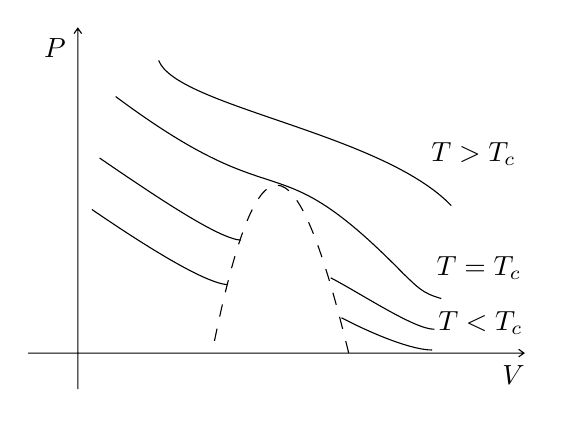
\begin{tikzpicture}[x=0.75pt,y=0.75pt,yscale=-0.37,xscale=0.37]
%uncomment if require: \path (0,476); %set diagram left start at 0, and has height of 476

%Shape: Axis 2D [id:dp5951100625553807]
\draw  (12.61,425) -- (658.18,425)(77.17,2) -- (77.17,472) (651.18,420) -- (658.18,425) -- (651.18,430) (72.17,9) -- (77.17,2) -- (82.17,9)  ;
%Curve Lines [id:da2126694468363458]
\draw    (563.5,233) .. controls (472.5,138) and (205.5,104) .. (182.5,44) ;


%Curve Lines [id:da8602998139648838]
\draw  [dash pattern={on 4.5pt off 4.5pt}]  (429.9,424.97) .. controls (359.9,136.97) and (310.9,129.97) .. (251.9,424.97) ;


%Shape: Boxed Bezier Curve [id:dp6932412254916785]
\draw    (501.5,322) .. controls (326.5,143) and (349.5,257) .. (126.5,91) ;


%Curve Lines [id:da8502267220518913]
\draw    (289.5,278) .. controls (260.5,276) and (181.5,223) .. (105.5,171) ;


%Curve Lines [id:da8746517244181468]
\draw    (272.5,336) .. controls (243.5,334) and (171.5,290) .. (95.5,238) ;


%Curve Lines [id:da4382617853232931]
\draw    (538.5,421) .. controls (512.5,421) and (462.5,401) .. (420.5,379) ;


%Curve Lines [id:da368608553657754]
\draw    (541.5,394) .. controls (515.5,394) and (448.5,349) .. (406.5,327) ;


%Curve Lines [id:da19861479220559797]
\draw    (550.5,354) .. controls (525.5,347) and (519.5,339) .. (501.5,322) ;



% Text Node
\draw (47.5,27.32) node [scale=1]  {$P$};
% Text Node
\draw (644.64,453.88) node [scale=1]  {$V$};
% Text Node
\draw (601.49,385.88) node [scale=1]  {$T< T_{c}$};
% Text Node
\draw (599.49,313.88) node [scale=1]  {$T=T_{c}$};
% Text Node
\draw (592.49,165.88) node [scale=1]  {$T >T_{c}$};


\end{tikzpicture}
    \label{fig:3_2_2} }
\end{minipage}
\caption{\label{fig:3_2} Description}
\end{figure}


In Figure \ref{fig:3_3} is shown the behaviour for a ferromagnetic system. Clearly \( M \neq 0 \) if \( H \neq 0 \). Recall that \emph{M} is the order parameter of the paramagnetic-ferromagnetic phase transition:
\begin{equation}
  H= 0 \Rightarrow \begin{cases}
    M \neq 0 & T < T_c   \\
    M \rightarrow 0 & T \rightarrow T_c^-
\end{cases}
  \label{eq:}
\end{equation}
 Consider \emph{ferromagnetic system}, we have \( \va{M} \rightarrow \va{H}   \) (magnetic field), while for \emph{ferro electric} we have \( \va{P} \rightarrow \va{E}   \) (electric field). For \emph{liquid crystals} \( Q_{\alpha \beta } \rightarrow \va{E},\va{H}   \), for \emph{fluid} \( V \rightarrow P \) (pressure) or \( rho \rightarrow \mu  \).
 \begin{remark}
 Note that \( \rho = \frac{N}{V} = \frac{1}{v} \) hence either \emph{N} or \emph{V} varies.
 \end{remark}



\begin{figure}[h!]
\centering


\tikzset{every picture/.style={line width=0.75pt}} %set default line width to 0.75pt

\begin{tikzpicture}[x=0.75pt,y=0.75pt,yscale=-0.7,xscale=0.7]
%uncomment if require: \path (0,476); %set diagram left start at 0, and has height of 476

%Shape: Axis 2D [id:dp5951100625553807]
\draw  (6.61,238.94) -- (652.18,238.94)(72.5,3) -- (72.5,473) (645.18,233.94) -- (652.18,238.94) -- (645.18,243.94) (67.5,10) -- (72.5,3) -- (77.5,10)  ;
%Curve Lines [id:da2126694468363458]
\draw    (582.5,278.94) .. controls (367.5,268.94) and (237.5,380.94) .. (127.5,471.94) ;


%Curve Lines [id:da8099781123736827]
\draw    (583.5,216.94) .. controls (448.5,202.94) and (228.5,87.94) .. (151.5,33.94) ;


%Curve Lines [id:da6865648324380681]
\draw [color={rgb, 255:red, 255; green, 0; blue, 0 }  ,draw opacity=1 ]   (71.5,99.94) .. controls (315.5,126.94) and (361.5,332.94) .. (72.5,397.94) ;


%Shape: Circle [id:dp406793341592669]
\draw  [color={rgb, 255:red, 255; green, 0; blue, 0 }  ,draw opacity=1 ][fill={rgb, 255:red, 255; green, 0; blue, 0 }  ,fill opacity=1 ] (267.06,237.97) .. controls (267.06,235.23) and (269.28,233) .. (272.03,233) .. controls (274.77,233) and (277,235.23) .. (277,237.97) .. controls (277,240.72) and (274.77,242.94) .. (272.03,242.94) .. controls (269.28,242.94) and (267.06,240.72) .. (267.06,237.97) -- cycle ;

% Text Node
\draw (47.5,27.32) node [scale=1.5]  {$M$};
% Text Node
\draw (626.64,258.88) node [scale=1.5]  {$T$};
% Text Node
\draw (492.49,372.88) node [scale=1]  {$H< 0$};
% Text Node
\draw (559.49,254.88) node [scale=1]  {$H=0$};
% Text Node
\draw (489.49,94.88) node [scale=1]  {$H >0$};
% Text Node
\draw (292.49,215.88) node [scale=1,color={rgb, 255:red, 253; green, 0; blue, 0 }  ,opacity=1 ]  {$T_{c}$};

\end{tikzpicture}


\caption{\label{fig:3_3} Description.}
\end{figure}

\section{Divergence of the responde functions at the critical point}
While at the critical point the order parameter goes to zero continuously as \( T \rightarrow T_c^- \), the responde function may develop divergences.
\begin{example}
In a fluid system since at \( T=T_c \) the curve \( P = P(V) \) develops an horizontal flex (Figure \ref{fig:3_2_2}), we have \( k_T = -\frac{1}{V} \qty(\pdv{V}{P} )_T  \rightarrow \infty  \). Similarly, in a magnetic since the curve is like Figure , we have \( \chi _T = \qty(\pdv{M}{H} )_T \underset{T \rightarrow  T_c}{\rightarrow } \infty   \)


\end{example}

\section{Thermodynamic classification of the phase transitions}
Thermodynamically one can distinguish two kinds of phase transitions:
\begin{enumerate}
\item Ones who develop latent heat.
\item Ones who do not develop latent heat. The entropy changes continuously at the transition.
\end{enumerate}
\subsection{Eherenfest classification}
The \emph{Eherenfest classification} is based on the behaviour of the derivatives of the thermodynamic potentials.

A phase transition is of order \emph{n} if all the \emph{n-1} derivatives are continuous and the \( n^{th} \) derivative displays a finite discontinuity.
\begin{example}
For instance, the first order transition \( S=-(\partial{G}/\partial{T}  )_P \) has finite discontinuity.
\end{example}
\begin{remark}
There are first order transitions where \emph{S} is continuous (no latent heat) but \( \rho  \) is discontinuous ( \( v = (\partial{G}/\partial{P}  )_T \) ).
\end{remark}
\begin{example}
Second order transition. The specific heat displays a finite jump, see Figure \ref{fig:3_04_3} in the conductor-superconductor transition.
\end{example}
Second order transition but with divergence. Consider the fluid-superfluid transition (or \( \lambda  \) transition ) of the \( \text{He}_4 \) (Figure \ref{fig:3_04_4}).



\begin{figure}[h!]
\begin{minipage}[c]{0.5\linewidth}
\centering
\subfloat[][]{
\tikzset{every picture/.style={line width=0.75pt}} %set default line width to 0.75pt

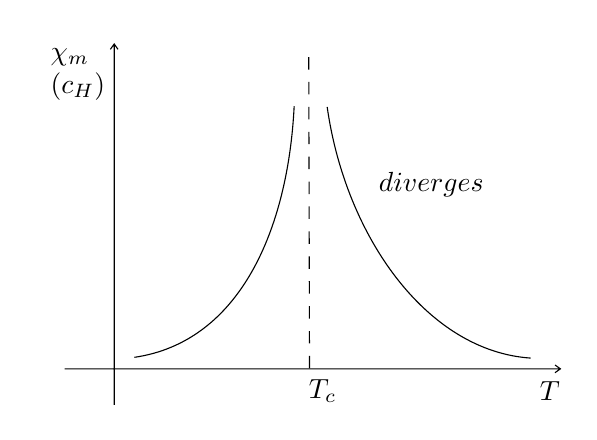
\begin{tikzpicture}[x=0.75pt,y=0.75pt,yscale=-0.37,xscale=0.37]
%uncomment if require: \path (0,476); %set diagram left start at 0, and has height of 476

%Shape: Axis 2D [id:dp5951100625553807]
\draw  (12.61,425) -- (658.18,425)(77.17,2) -- (77.17,472) (651.18,420) -- (658.18,425) -- (651.18,430) (72.17,9) -- (77.17,2) -- (82.17,9)  ;
%Straight Lines [id:da5293875835625754]
\draw  [dash pattern={on 4.5pt off 4.5pt}]  (330.5,19) -- (331.5,425) ;


%Curve Lines [id:da44190238222280653]
\draw    (103.5,410) .. controls (240.5,390) and (303.5,244) .. (311.5,83) ;


%Curve Lines [id:da7750908509461275]
\draw    (619.5,411) .. controls (484.5,402) and (378.5,253) .. (354.5,84) ;



% Text Node
\draw (644.64,453.88) node [scale=1]  {$T$};
% Text Node
\draw (348.49,453.88) node [scale=1]  {$T_{c}$};
% Text Node
\draw (30,36) node [scale=1]  {$ \begin{array}{l}
\chi _{m}\\
( c_{H})
\end{array}$};
\draw (490,185) node [scale=1]  {$diverges$};

\end{tikzpicture}
    \label{fig:} }
\end{minipage}
\begin{minipage}[]{0.5\linewidth}
\centering
\subfloat[][Liquid gas \( k_T = - \frac{1}{V} \pdv{V}{P}  \) ]{
\tikzset{every picture/.style={line width=0.75pt}} %set default line width to 0.75pt

\begin{tikzpicture}[x=0.75pt,y=0.75pt,yscale=-0.37,xscale=0.37]
%uncomment if require: \path (0,476); %set diagram left start at 0, and has height of 476

%Shape: Axis 2D [id:dp5951100625553807]
\draw  (12.61,425) -- (658.18,425)(77.17,2) -- (77.17,472) (651.18,420) -- (658.18,425) -- (651.18,430) (72.17,9) -- (77.17,2) -- (82.17,9)  ;
%Straight Lines [id:da5293875835625754]
\draw  [dash pattern={on 4.5pt off 4.5pt}]  (330.5,19) -- (331.5,425) ;


%Curve Lines [id:da7750908509461275]
\draw    (550.5,348) .. controls (501.5,255) and (456.5,217) .. (395.5,213) .. controls (334.5,209) and (220.5,205) .. (125.5,94) ;


%Shape: Circle [id:dp9976635914729922]
\draw  [fill={rgb, 255:red, 0; green, 0; blue, 0 }  ,fill opacity=1 ] (326,206.5) .. controls (326,204.02) and (328.01,202) .. (330.5,202) .. controls (332.98,202) and (335,204.02) .. (335,206.5) .. controls (335,208.99) and (332.98,211) .. (330.5,211) .. controls (328.01,211) and (326,208.99) .. (326,206.5) -- cycle ;

% Text Node
\draw (644.64,453.88) node [scale=1]  {$T$};
% Text Node
\draw (336.49,449.88) node [scale=1]  {$T_{c}$};
% Text Node
\draw (41,36) node [scale=1]  {$c_{p}$};
% Text Node
\draw (433,163) node   {$flex\ point$};


\end{tikzpicture}
    \label{fig:} }
\end{minipage}
\\
\begin{minipage}[c]{0.5\linewidth}
\centering
\subfloat[][2° order phase transition]{

\tikzset{every picture/.style={line width=0.75pt}} %set default line width to 0.75pt

\begin{tikzpicture}[x=0.75pt,y=0.75pt,yscale=-0.37,xscale=0.37]
%uncomment if require: \path (0,476); %set diagram left start at 0, and has height of 476

%Shape: Axis 2D [id:dp5951100625553807]
\draw  (12.61,425) -- (658.18,425)(77.17,2) -- (77.17,472) (651.18,420) -- (658.18,425) -- (651.18,430) (72.17,9) -- (77.17,2) -- (82.17,9)  ;
%Straight Lines [id:da5293875835625754]
\draw  [dash pattern={on 4.5pt off 4.5pt}]  (330.5,19) -- (331.5,425) ;


%Curve Lines [id:da44190238222280653]
\draw    (103.5,410) .. controls (240.5,390) and (290.5,241) .. (331.5,84) ;


%Curve Lines [id:da7750908509461275]
\draw    (619.5,411) .. controls (484.5,402) and (406.5,367) .. (330.5,213) ;



% Text Node
\draw (644.64,453.88) node [scale=1]  {$T$};
% Text Node
\draw (348.49,453.88) node [scale=1]  {$T_{s}$};
% Text Node
\draw (41,36) node [scale=1]  {$c_{p}$};
% Text Node
\draw (408,185) node   {$jump$};


\end{tikzpicture}
    \label{fig:3_04_3} }
\end{minipage}
\begin{minipage}[]{0.5\linewidth}
\centering
\subfloat[][Superfluid in \( \lambda\)-transition ]{
\tikzset{every picture/.style={line width=0.75pt}} %set default line width to 0.75pt

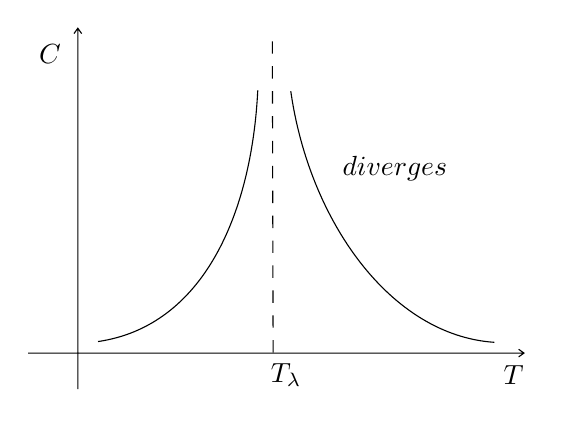
\begin{tikzpicture}[x=0.75pt,y=0.75pt,yscale=-0.37,xscale=0.37]
%uncomment if require: \path (0,476); %set diagram left start at 0, and has height of 476

%Shape: Axis 2D [id:dp5951100625553807]
\draw  (12.61,425) -- (658.18,425)(77.17,2) -- (77.17,472) (651.18,420) -- (658.18,425) -- (651.18,430) (72.17,9) -- (77.17,2) -- (82.17,9)  ;
%Straight Lines [id:da5293875835625754]
\draw  [dash pattern={on 4.5pt off 4.5pt}]  (330.5,19) -- (331.5,425) ;


%Curve Lines [id:da44190238222280653]
\draw    (103.5,410) .. controls (240.5,390) and (303.5,244) .. (311.5,83) ;


%Curve Lines [id:da7750908509461275]
\draw    (619.5,411) .. controls (484.5,402) and (378.5,253) .. (354.5,84) ;



% Text Node
\draw (644.64,453.88) node [scale=1]  {$T$};
% Text Node
\draw (348.49,453.88) node [scale=1]  {$T_{\lambda }$};
% Text Node
\draw (41,36) node [scale=1]  {$C$};
\draw (490,185) node [scale=1]  {$diverges$};

\end{tikzpicture}
    \label{fig:3_04_4} }
\end{minipage}
\caption{\label{fig:} Description}
\end{figure}

\subsection{Modern classification}
A phase transition is of the first order if exists a finite discontinuity in either one or more partial derivatives of the thermodynamic potentials. If instead the first derivatives are all continuous but the second are either discontinuous or infinite one talks of continuous transitions.
A critical point is a continuous transition.

\section{Critical exponents}
At the critical point response functions may diverge. How are these divergence?
In general, when you are close to \( T_c \), there are singolarities. Now, we can ask, how the curve diverges? What is the behaviour close to the critical point? Power law, so which are the values of these critical exponents? The notion of \emph{critical exponent} describes the behaviour of the order parameter and the responde functions in proximity of the critical point.
In order to answer to these questions, let us define:

\begin{bluebox}
\begin{definition}[\textbf{Critical Exponent} (or \emph{Scale Exponent})] \
Define the adimensional parameter measuring the distance from the critical point\( t \equiv \frac{T-T_c}{T_c} \), the \emph{Critical Exponent} \( \lambda  \) associated to the function \( F(t) \) is defined as:
\begin{equation}
  \lambda _{\pm} = \lim_{t \rightarrow 0^{\pm}} \frac{\ln{\abs{F(t)} } }{\ln{\abs{t} } }
  \label{eq:}
\end{equation}
\end{definition}
\end{bluebox}
We note that it behaves like a power low and that one can also write the \textbf{power law}:
\begin{equation}
  F(t) \overset{t \rightarrow  0^{\pm}}{\sim } \abs{t}^{\lambda _{\pm}}
  \label{eq:}
\end{equation}
More generally, for \( t \ll 1 \):
\begin{equation}
  F(t) = A \abs{t}^{\lambda _{\pm}} ( 1 + bt^{\lambda _1}+ \dots) \quad \lambda _1 > 0
  \label{eq:}
\end{equation}
where all other terms are less important.
\begin{bluebox}
\begin{definition}[Thermodynamic critical exponents]\
\begin{itemize}
\item \textbf{Exponent \( \beta \) }: tells how the order parameter goes to zero.
Consider Figure \ref{fig:3_4_1}, we have \( M \overset{t \rightarrow  0^-}{\sim} (-t)^{\beta }  \). No sense in going from above where it stays 0.

\item \textbf{Exponent \( \gamma _{\pm}  \) } (suscettibility): related to the response function. Consider Figure \ref{fig:3_4_2}, we have \( \chi _T \overset{t \rightarrow 0^{\pm}}{\sim} \abs{t}^{-\gamma _{\pm} }   \). In principle, the value of \( \gamma   \) can depend on the sign of \emph{t} i.e.   \( \gamma ^+ \neq \gamma ^-  \), but they are the same in reality and we have \( \gamma ^+ = \gamma ^- = \gamma     \).

\item \textbf{Exponent \( \alpha _{\pm} \) }: how specific heat diverges (second order derivative in respect of \emph{T} ). For instance see Figure \ref{fig:3_4_3}, we have \( c_H \sim \abs{t}^{-\alpha _{\pm}}  \).

\item \textbf{Exponent \( \delta   \)}: in this case one consider the isotherm \( T =T_c \) and look for the behaviour of \emph{M} at the critical point at small \emph{H} (or viceversa).  The result is \( M \sim H^{1/\delta } \).
In Figure \ref{fig:3_4_4}, \( H \sim \abs{M}^{\delta } \text{sign} (M)  \).

\end{itemize}
\end{definition}
\end{bluebox}



\begin{figure}[h!]
\begin{minipage}[c]{0.5\linewidth}
\centering
\subfloat[][Exponent \( \beta  \) ]{
\tikzset{every picture/.style={line width=0.75pt}} %set default line width to 0.75pt

\begin{tikzpicture}[x=0.75pt,y=0.75pt,yscale=-0.37,xscale=0.37]
%uncomment if require: \path (0,476); %set diagram left start at 0, and has height of 476

%Shape: Axis 2D [id:dp5951100625553807]
\draw  (12.61,425) -- (658.18,425)(77.17,2) -- (77.17,472) (651.18,420) -- (658.18,425) -- (651.18,430) (72.17,9) -- (77.17,2) -- (82.17,9)  ;
%Curve Lines [id:da7750908509461275]
\draw    (470.5,424) .. controls (463.5,331) and (450.5,257) .. (365.5,194) .. controls (280.5,131) and (253.5,117) .. (77.5,92) ;



% Text Node
\draw (644.64,453.88) node [scale=1]  {$T$};
% Text Node
\draw (471.49,448.88) node [scale=1]  {$T_{c}$};
% Text Node
\draw (41,36) node [scale=1]  {$M$};
% Text Node
\draw (306,102) node   {$H=0$};


\end{tikzpicture}
    \label{fig:3_4_1} }
\end{minipage}
\begin{minipage}[]{0.5\linewidth}
\centering
\subfloat[][Exponent \( \gamma_{\pm}  \) ]{
\tikzset{every picture/.style={line width=0.75pt}} %set default line width to 0.75pt

\begin{tikzpicture}[x=0.75pt,y=0.75pt,yscale=-0.37,xscale=0.37]
%uncomment if require: \path (0,476); %set diagram left start at 0, and has height of 476

%Shape: Axis 2D [id:dp5951100625553807]
\draw  (12.61,425) -- (658.18,425)(77.17,2) -- (77.17,472) (651.18,420) -- (658.18,425) -- (651.18,430) (72.17,9) -- (77.17,2) -- (82.17,9)  ;
%Straight Lines [id:da5293875835625754]
\draw  [dash pattern={on 4.5pt off 4.5pt}]  (330.5,19) -- (331.5,425) ;


%Curve Lines [id:da44190238222280653]
\draw    (103.5,410) .. controls (240.5,390) and (303.5,244) .. (311.5,83) ;


%Curve Lines [id:da7750908509461275]
\draw    (619.5,411) .. controls (484.5,402) and (378.5,253) .. (354.5,84) ;



% Text Node
\draw (644.64,453.88) node [scale=1]  {$T$};
% Text Node
\draw (348.49,453.88) node [scale=1]  {$T_{c}$};
% Text Node
\draw (30,36) node [scale=1]  {$\chi$};
\draw (490,185) node [scale=1]  {$H=0$};

\end{tikzpicture}
    \label{fig:3_4_2} }
\end{minipage}
\\
\begin{minipage}[c]{0.5\linewidth}
\centering
\subfloat[][Exponent \( \alpha _{\pm} \) ]{
\tikzset{every picture/.style={line width=0.75pt}} %set default line width to 0.75pt

\begin{tikzpicture}[x=0.75pt,y=0.75pt,yscale=-0.37,xscale=0.37]
%uncomment if require: \path (0,476); %set diagram left start at 0, and has height of 476

%Shape: Axis 2D [id:dp5951100625553807]
\draw  (12.61,425) -- (658.18,425)(77.17,2) -- (77.17,472) (651.18,420) -- (658.18,425) -- (651.18,430) (72.17,9) -- (77.17,2) -- (82.17,9)  ;
%Straight Lines [id:da5293875835625754]
\draw  [dash pattern={on 4.5pt off 4.5pt}]  (330.5,19) -- (331.5,425) ;


%Curve Lines [id:da44190238222280653]
\draw    (103.5,410) .. controls (240.5,390) and (303.5,244) .. (311.5,83) ;


%Curve Lines [id:da7750908509461275]
\draw    (619.5,411) .. controls (484.5,402) and (378.5,253) .. (354.5,84) ;



% Text Node
\draw (644.64,453.88) node [scale=1]  {$T$};
% Text Node
\draw (348.49,453.88) node [scale=1]  {$T_{c}$};
% Text Node
\draw (30,36) node [scale=1]  {$c_{H}$};
\draw (490,185) node [scale=1]  {$H=0$};

\end{tikzpicture}
    \label{fig:3_4_3} }
\end{minipage}
\begin{minipage}[]{0.5\linewidth}
\centering
\subfloat[][Exponent \( \gamma   \) ]{
\tikzset{every picture/.style={line width=0.75pt}} %set default line width to 0.75pt

\begin{tikzpicture}[x=0.75pt,y=0.75pt,yscale=-0.37,xscale=0.37]
%uncomment if require: \path (0,476); %set diagram left start at 0, and has height of 476

%Shape: Axis 2D [id:dp5951100625553807]
\draw  (12.61,242) -- (658.18,242)(329.5,2) -- (329.5,472) (651.18,237) -- (658.18,242) -- (651.18,247) (324.5,9) -- (329.5,2) -- (334.5,9)  ;
%Curve Lines [id:da0018844471566330512]
\draw    (100.5,400) .. controls (207.5,400) and (243.5,430) .. (329.5,242) .. controls (415.5,54) and (537.5,101) .. (571.5,94) ;



% Text Node
\draw (623.64,276.88) node [scale=1]  {$H$};
% Text Node
\draw (497.49,60.88) node [scale=1]  {$T=T_{c}$};
% Text Node
\draw (291,22) node [scale=1]  {$M$};


\end{tikzpicture}
    \label{fig:3_4_4} }
\end{minipage}
\caption{\label{fig:} Description}
\end{figure}


\subsection{Law of the corresponding states}
The system displays correlation at very long distance, these goes to the size of the system when \( T \rightarrow T_c \). We are talking about long range correlation. The \emph{correlation function} is \( \xi \sim t^{-\nu } \).
For instance, consider a polymer as in Figure \ref{fig:3_5}.

The critical exponents are more interesting than \( T_c \) since their values do not depend on microscopic details but only on few parameters such as the space dimension \emph{d} and the symmetry of the system. One of the first experimental evidence of this universality was given by the work of Guggenheim on the coexistence curves of \emph{g} different fluids: A, Kn, $\chi_e$, Ne, $N_2$, $CO_2$ and $O_2$. By plotting \( T/T_c \) versus \( \rho /\rho _c \) (Figure \ref{fig:3_6}) he found that all the data collapse on the same curve, i.e. different sets of data fit the  same function. Moreover for \( t \rightarrow 0 \):
\begin{equation}
  (\rho _l - \rho _c) \sim (-t)^{\beta}
  \label{eq:}
\end{equation}
and \( \beta \sim 1/3 \approx 0.335 \). If you do the same for a string ferromagnetic is 1/3 too.
\begin{remark}
The law of corresponding states gives a universal liquid-gas coexistence curve.
\end{remark}
The law is quite remarkable considering the spread in the values of critical parameters of the substances considered.

\subsection{Thermodynamic inequalities between critical exponents}
\subsubsection{Rushbrocke inequality}
Remember the relation between response functions:

\begin{equation}
  \begin{cases}
   k_T (c_p-c_v)=T v \alpha ^2 = T v \frac{1}{v^2} \qty(\pdv{v}{T} )^2_P = T \frac{1}{v} \qty(\pdv{v}{T} )^2_P  \\
   \chi _T (c_H-c_M) = T \qty(\pdv{M}{T} )^2_H
  \end{cases}
\label{eq:}
\end{equation}
from the thermodynamic stability we have \( c_M \geq 0, \chi _T \geq 0  \).
Hence from the previous relation we have
\begin{equation}
   c_H \geq \frac{T}{\chi _T} \qty(\pdv{M}{T} )^2
  \label{eq:}
\end{equation}
On the other hand, for \( T \rightarrow T_c^- \) and \( H=0 \) we have
\begin{equation}
  \begin{cases}
   c_H \sim (-t)^{-\alpha }\\
   \chi _T \sim (-t)^{-\gamma  }
  \end{cases}
\label{eq:}
\end{equation}
Therefore \( M \sim (-t)^{\beta } \), which implies \( \qty( \pdv{M}{T})_{H=0} \sim (-t)^{\beta -1} \).
Since the inequality is valid for all temperature \emph{T} it follows
\begin{equation}
  B (T_c - T)^{-\alpha } \ge B' T \frac{[(T_c - T)^{\beta -1}]^2}{(T_c-T)^{-\gamma  }}
  \label{eq:}
\end{equation}
with \( B,B' > 0 \). Take the limit \( T \rightarrow T_c^- \) we have:
\begin{equation}
  \lim_{T \rightarrow T_c^-} (T_c - T)^{2- \alpha - 2 \beta - \gamma  } \ge \frac{B' T}{B} > 0
  \label{eq:}
\end{equation}
Since the left hand side must be strictly greater than zero we have the \textcolor{blue}{\textbf{RushBrook inequality}}:

\begin{empheq}[box=\myyellowbox]{equation}
\alpha + 2 \beta  + \gamma \geq 2
\end{empheq}
Is obtained from the convexity property (in \emph{T} and \emph{V}) of the Helmolds free energy and from \( A \sim t^{2- \alpha } \):
\begin{equation}
  \Rightarrow \alpha + \beta (1+\delta ) \ge 2
  \label{eq:}
\end{equation}









\begin{figure}[h!]
\begin{minipage}[c]{0.5\linewidth}

\subfloat[][Description]{   \centering
\tikzset{every picture/.style={line width=0.75pt}} %set default line width to 0.75pt

\begin{tikzpicture}[x=0.75pt,y=0.75pt,yscale=-0.37,xscale=0.37]
%uncomment if require: \path (0,300); %set diagram left start at 0, and has height of 300

%Curve Lines [id:da3452922115663215]
\draw    (7.5,293) .. controls (206.5,-11) and (350.5,204) .. (645.5,37) ;


%Shape: Circle [id:dp7203554451656493]
\draw  [fill={rgb, 255:red, 0; green, 0; blue, 0 }  ,fill opacity=1 ] (4.86,286.36) .. controls (4.86,282.15) and (8.28,278.73) .. (12.5,278.73) .. controls (16.72,278.73) and (20.14,282.15) .. (20.14,286.36) .. controls (20.14,290.58) and (16.72,294) .. (12.5,294) .. controls (8.28,294) and (4.86,290.58) .. (4.86,286.36) -- cycle ;
%Shape: Circle [id:dp5606402691740692]
\draw  [fill={rgb, 255:red, 0; green, 0; blue, 0 }  ,fill opacity=1 ] (63.86,209.36) .. controls (63.86,205.15) and (67.28,201.73) .. (71.5,201.73) .. controls (75.72,201.73) and (79.14,205.15) .. (79.14,209.36) .. controls (79.14,213.58) and (75.72,217) .. (71.5,217) .. controls (67.28,217) and (63.86,213.58) .. (63.86,209.36) -- cycle ;
%Shape: Circle [id:dp08848917685644386]
\draw  [fill={rgb, 255:red, 0; green, 0; blue, 0 }  ,fill opacity=1 ] (135.86,152.36) .. controls (135.86,148.15) and (139.28,144.73) .. (143.5,144.73) .. controls (147.72,144.73) and (151.14,148.15) .. (151.14,152.36) .. controls (151.14,156.58) and (147.72,160) .. (143.5,160) .. controls (139.28,160) and (135.86,156.58) .. (135.86,152.36) -- cycle ;
%Shape: Circle [id:dp2975813160236622]
\draw  [fill={rgb, 255:red, 0; green, 0; blue, 0 }  ,fill opacity=1 ] (219.86,120.36) .. controls (219.86,116.15) and (223.28,112.73) .. (227.5,112.73) .. controls (231.72,112.73) and (235.14,116.15) .. (235.14,120.36) .. controls (235.14,124.58) and (231.72,128) .. (227.5,128) .. controls (223.28,128) and (219.86,124.58) .. (219.86,120.36) -- cycle ;
%Shape: Circle [id:dp10353996653211406]
\draw  [fill={rgb, 255:red, 0; green, 0; blue, 0 }  ,fill opacity=1 ] (321.86,111.36) .. controls (321.86,107.15) and (325.28,103.73) .. (329.5,103.73) .. controls (333.72,103.73) and (337.14,107.15) .. (337.14,111.36) .. controls (337.14,115.58) and (333.72,119) .. (329.5,119) .. controls (325.28,119) and (321.86,115.58) .. (321.86,111.36) -- cycle ;
%Shape: Circle [id:dp5932331084017816]
\draw  [fill={rgb, 255:red, 0; green, 0; blue, 0 }  ,fill opacity=1 ] (433.86,106.36) .. controls (433.86,102.15) and (437.28,98.73) .. (441.5,98.73) .. controls (445.72,98.73) and (449.14,102.15) .. (449.14,106.36) .. controls (449.14,110.58) and (445.72,114) .. (441.5,114) .. controls (437.28,114) and (433.86,110.58) .. (433.86,106.36) -- cycle ;
%Shape: Circle [id:dp0026977079762487977]
\draw  [fill={rgb, 255:red, 0; green, 0; blue, 0 }  ,fill opacity=1 ] (536.86,82.36) .. controls (536.86,78.15) and (540.28,74.73) .. (544.5,74.73) .. controls (548.72,74.73) and (552.14,78.15) .. (552.14,82.36) .. controls (552.14,86.58) and (548.72,90) .. (544.5,90) .. controls (540.28,90) and (536.86,86.58) .. (536.86,82.36) -- cycle ;
%Shape: Circle [id:dp7071423275830327]
\draw  [fill={rgb, 255:red, 0; green, 0; blue, 0 }  ,fill opacity=1 ] (637.86,37) .. controls (637.86,32.78) and (641.28,29.36) .. (645.5,29.36) .. controls (649.72,29.36) and (653.14,32.78) .. (653.14,37) .. controls (653.14,41.22) and (649.72,44.64) .. (645.5,44.64) .. controls (641.28,44.64) and (637.86,41.22) .. (637.86,37) -- cycle ;

% Text Node
\draw (107,64) node [scale=2.074]  {$N$};


\end{tikzpicture}
    \label{fig:3_5} }
\end{minipage}
\begin{minipage}[]{0.5\linewidth}
\centering
\subfloat[][Description]{   \centering
\tikzset{every picture/.style={line width=0.75pt}} %set default line width to 0.75pt

\begin{tikzpicture}[x=0.75pt,y=0.75pt,yscale=-0.37,xscale=0.37]
%uncomment if require: \path (0,476); %set diagram left start at 0, and has height of 476

%Shape: Axis 2D [id:dp5951100625553807]
\draw  (12.61,425) -- (658.18,425)(77.17,2) -- (77.17,472) (651.18,420) -- (658.18,425) -- (651.18,430) (72.17,9) -- (77.17,2) -- (82.17,9)  ;
%Curve Lines [id:da8602998139648838]
\draw    (540.5,425) .. controls (468.5,-33) and (195.1,-68.97) .. (119.5,424) ;


%Straight Lines [id:da9201699988131803]
\draw  [dash pattern={on 4.5pt off 4.5pt}]  (326.5,67) -- (326.5,425) ;


%Shape: Circle [id:dp2338308227400978]
\draw  [color={rgb, 255:red, 255; green, 0; blue, 0 }  ,draw opacity=1 ][fill={rgb, 255:red, 255; green, 0; blue, 0 }  ,fill opacity=1 ] (124.9,365.08) .. controls (124.9,362.83) and (126.73,361) .. (128.99,361) .. controls (131.24,361) and (133.07,362.83) .. (133.07,365.08) .. controls (133.07,367.34) and (131.24,369.17) .. (128.99,369.17) .. controls (126.73,369.17) and (124.9,367.34) .. (124.9,365.08) -- cycle ;
%Shape: Circle [id:dp8006128175966643]
\draw  [color={rgb, 255:red, 255; green, 0; blue, 0 }  ,draw opacity=1 ][fill={rgb, 255:red, 255; green, 0; blue, 0 }  ,fill opacity=1 ] (146.9,281.08) .. controls (146.9,278.83) and (148.73,277) .. (150.99,277) .. controls (153.24,277) and (155.07,278.83) .. (155.07,281.08) .. controls (155.07,283.34) and (153.24,285.17) .. (150.99,285.17) .. controls (148.73,285.17) and (146.9,283.34) .. (146.9,281.08) -- cycle ;
%Shape: Circle [id:dp23793761340225705]
\draw  [color={rgb, 255:red, 255; green, 0; blue, 0 }  ,draw opacity=1 ][fill={rgb, 255:red, 255; green, 0; blue, 0 }  ,fill opacity=1 ] (170.9,210.08) .. controls (170.9,207.83) and (172.73,206) .. (174.99,206) .. controls (177.24,206) and (179.07,207.83) .. (179.07,210.08) .. controls (179.07,212.34) and (177.24,214.17) .. (174.99,214.17) .. controls (172.73,214.17) and (170.9,212.34) .. (170.9,210.08) -- cycle ;
%Shape: Circle [id:dp6439712554976472]
\draw  [color={rgb, 255:red, 255; green, 0; blue, 0 }  ,draw opacity=1 ][fill={rgb, 255:red, 255; green, 0; blue, 0 }  ,fill opacity=1 ] (205.9,147.08) .. controls (205.9,144.83) and (207.73,143) .. (209.99,143) .. controls (212.24,143) and (214.07,144.83) .. (214.07,147.08) .. controls (214.07,149.34) and (212.24,151.17) .. (209.99,151.17) .. controls (207.73,151.17) and (205.9,149.34) .. (205.9,147.08) -- cycle ;
%Shape: Circle [id:dp09113196346350672]
\draw  [color={rgb, 255:red, 255; green, 0; blue, 0 }  ,draw opacity=1 ][fill={rgb, 255:red, 255; green, 0; blue, 0 }  ,fill opacity=1 ] (264.9,84.08) .. controls (264.9,81.83) and (266.73,80) .. (268.99,80) .. controls (271.24,80) and (273.07,81.83) .. (273.07,84.08) .. controls (273.07,86.34) and (271.24,88.17) .. (268.99,88.17) .. controls (266.73,88.17) and (264.9,86.34) .. (264.9,84.08) -- cycle ;
%Shape: Circle [id:dp9797333610021878]
\draw  [color={rgb, 255:red, 255; green, 0; blue, 0 }  ,draw opacity=1 ][fill={rgb, 255:red, 255; green, 0; blue, 0 }  ,fill opacity=1 ] (322.42,67) .. controls (322.42,64.74) and (324.24,62.92) .. (326.5,62.92) .. controls (328.76,62.92) and (330.58,64.74) .. (330.58,67) .. controls (330.58,69.26) and (328.76,71.08) .. (326.5,71.08) .. controls (324.24,71.08) and (322.42,69.26) .. (322.42,67) -- cycle ;
%Shape: Circle [id:dp6529970568279684]
\draw  [color={rgb, 255:red, 255; green, 0; blue, 0 }  ,draw opacity=1 ][fill={rgb, 255:red, 255; green, 0; blue, 0 }  ,fill opacity=1 ] (407.9,108.08) .. controls (407.9,105.83) and (409.73,104) .. (411.99,104) .. controls (414.24,104) and (416.07,105.83) .. (416.07,108.08) .. controls (416.07,110.34) and (414.24,112.17) .. (411.99,112.17) .. controls (409.73,112.17) and (407.9,110.34) .. (407.9,108.08) -- cycle ;
%Shape: Circle [id:dp9000295114661184]
\draw  [color={rgb, 255:red, 255; green, 0; blue, 0 }  ,draw opacity=1 ][fill={rgb, 255:red, 255; green, 0; blue, 0 }  ,fill opacity=1 ] (452.9,164.08) .. controls (452.9,161.83) and (454.73,160) .. (456.99,160) .. controls (459.24,160) and (461.07,161.83) .. (461.07,164.08) .. controls (461.07,166.34) and (459.24,168.17) .. (456.99,168.17) .. controls (454.73,168.17) and (452.9,166.34) .. (452.9,164.08) -- cycle ;
%Shape: Circle [id:dp9331849007810008]
\draw  [color={rgb, 255:red, 255; green, 0; blue, 0 }  ,draw opacity=1 ][fill={rgb, 255:red, 255; green, 0; blue, 0 }  ,fill opacity=1 ] (485.9,234.08) .. controls (485.9,231.83) and (487.73,230) .. (489.99,230) .. controls (492.24,230) and (494.07,231.83) .. (494.07,234.08) .. controls (494.07,236.34) and (492.24,238.17) .. (489.99,238.17) .. controls (487.73,238.17) and (485.9,236.34) .. (485.9,234.08) -- cycle ;
%Shape: Circle [id:dp5850866249072337]
\draw  [color={rgb, 255:red, 255; green, 0; blue, 0 }  ,draw opacity=1 ][fill={rgb, 255:red, 255; green, 0; blue, 0 }  ,fill opacity=1 ] (514.9,317.08) .. controls (514.9,314.83) and (516.73,313) .. (518.99,313) .. controls (521.24,313) and (523.07,314.83) .. (523.07,317.08) .. controls (523.07,319.34) and (521.24,321.17) .. (518.99,321.17) .. controls (516.73,321.17) and (514.9,319.34) .. (514.9,317.08) -- cycle ;
%Shape: Rectangle [id:dp7713336659871322]
\draw  [color={rgb, 255:red, 47; green, 53; blue, 87 }  ,draw opacity=1 ] (133,323) -- (142.98,323) -- (142.98,332.97) -- (133,332.97) -- cycle ;
%Shape: Rectangle [id:dp5637140961870309]
\draw  [color={rgb, 255:red, 47; green, 53; blue, 87 }  ,draw opacity=1 ] (159,237) -- (168.98,237) -- (168.98,246.97) -- (159,246.97) -- cycle ;
%Shape: Rectangle [id:dp7221266665867194]
\draw  [color={rgb, 255:red, 47; green, 53; blue, 87 }  ,draw opacity=1 ] (190,169) -- (199.98,169) -- (199.98,178.97) -- (190,178.97) -- cycle ;
%Shape: Rectangle [id:dp20263135432878354]
\draw  [color={rgb, 255:red, 47; green, 53; blue, 87 }  ,draw opacity=1 ] (230,109) -- (239.98,109) -- (239.98,118.97) -- (230,118.97) -- cycle ;
%Shape: Rectangle [id:dp7863774801349238]
\draw  [color={rgb, 255:red, 47; green, 53; blue, 87 }  ,draw opacity=1 ] (293,68) -- (302.98,68) -- (302.98,77.97) -- (293,77.97) -- cycle ;
%Shape: Rectangle [id:dp7641507230563557]
\draw  [color={rgb, 255:red, 47; green, 53; blue, 87 }  ,draw opacity=1 ] (370,75) -- (379.98,75) -- (379.98,84.97) -- (370,84.97) -- cycle ;
%Shape: Rectangle [id:dp15909977481521642]
\draw  [color={rgb, 255:red, 47; green, 53; blue, 87 }  ,draw opacity=1 ] (432,132) -- (441.98,132) -- (441.98,141.97) -- (432,141.97) -- cycle ;
%Shape: Rectangle [id:dp5185657164131019]
\draw  [color={rgb, 255:red, 47; green, 53; blue, 87 }  ,draw opacity=1 ] (471,196) -- (480.98,196) -- (480.98,205.97) -- (471,205.97) -- cycle ;
%Shape: Rectangle [id:dp17193812816873077]
\draw  [color={rgb, 255:red, 47; green, 53; blue, 87 }  ,draw opacity=1 ] (502,276) -- (511.98,276) -- (511.98,285.97) -- (502,285.97) -- cycle ;
%Shape: Rectangle [id:dp7377879387307478]
\draw  [color={rgb, 255:red, 47; green, 53; blue, 87 }  ,draw opacity=1 ] (525,361) -- (534.98,361) -- (534.98,370.97) -- (525,370.97) -- cycle ;

% Text Node
\draw (43.5,30.32) node [scale=1]  {$\frac{\rho }{\rho _{c}}$};
% Text Node
\draw (610.64,452.88) node [scale=1]  {$T/T_{c}$};
% Text Node
\draw (355.64,451.88) node [scale=1]  {$1=T_{c} /T_{c}$};

\end{tikzpicture}
    \label{fig:3_6} }
\end{minipage}
\caption{\label{fig:} }
\end{figure}




















\end{document}
